\section{Компьютерные эксперименты}
% \subsection{Параметры модели и оценок}
% В ходе экспериментов использовались следующие параметры модели:
% \begin{center}
%     \begin{tabular}{|p{5cm}|p{5cm}|}
%         \hline
%         \multicolumn{2}{|c|}{Параметры программы} \\
%         \hline
%         Переменная&значение\\
%         \hline
%         Размер выборки $N$& 1000\\
%         \hline
%         Доля выбросов $\widetilde{\varepsilon}$& 0.08\\
%         \hline
%         Параметры регрессии $\beta$& $(90,4)$\\
%         \hline
%         Регрессоры $x_i$ & $\sim U(-5,5)$\\
%         \hline
%         $\varepsilon_i$&$\sim N(0,16)$\\
%         \hline
%         $\eta_i$&$\sim N(100,100)$\\
%         \hline
%         Величина $K$ из пункта 2.3 курсового проекта &$10$\\
%         \hline
%     \end{tabular},
% \end{center}
% \newpage

\subsection{Сравнительный анализ построенной оценки с альтернативной}
\subsubsection{Эксперимент с изменением объема выборки}
В следующем эксперименте был произведен сравнительный анализ вариаций ОМП-оценок с МНК оценками в зависимости от объема выборки.

Объем выборки $N$ изменялся от $N_1=100$ до $N_2=500$, при этом выборка дополнялась, а не генерировалась новая. Использовалась модель линейной регрессии. Доля выбросов была постоянна и равнялась $\widetilde{\varepsilon}=0.08$. Параметры регрессии были постоянными и равнялись $\beta=(90,4)^T$. 
Регрессоры $x_i$ были из равномерного распределения $U(-5,5)$, ошибки эспериментов $\varepsilon_i\sim \mathcal{N}(0,16)$.

\begin{center}
    \captionof{table}{Параметры модели и оценок}\label{tab1}
    \begin{tabular}{|p{5cm}|p{5cm}|}
        \hline
        \multicolumn{2}{|c|}{Параметры программы} \\
        \hline
        Переменная&значение\\
        \hline
        Размер выборки $N$& от 100 до 500\\
        \hline
        Доля выбросов $\widetilde{\varepsilon}$& 0.08\\
        \hline
        Параметры регрессии $\beta$& $(90,4)$\\
        \hline
        Регрессоры $x_i$ & $\sim U(-5,5)$\\
        \hline
        $\varepsilon_i$&$\sim \mathcal{N}(0,16)$\\
        \hline
        $\eta_i$&$\sim \mathcal{N}(100,100)$\\
        \hline
        Величина $K$  &$10$\\
        \hline
    \end{tabular},
\end{center}
\begin{figure}[h!]
    \centering
    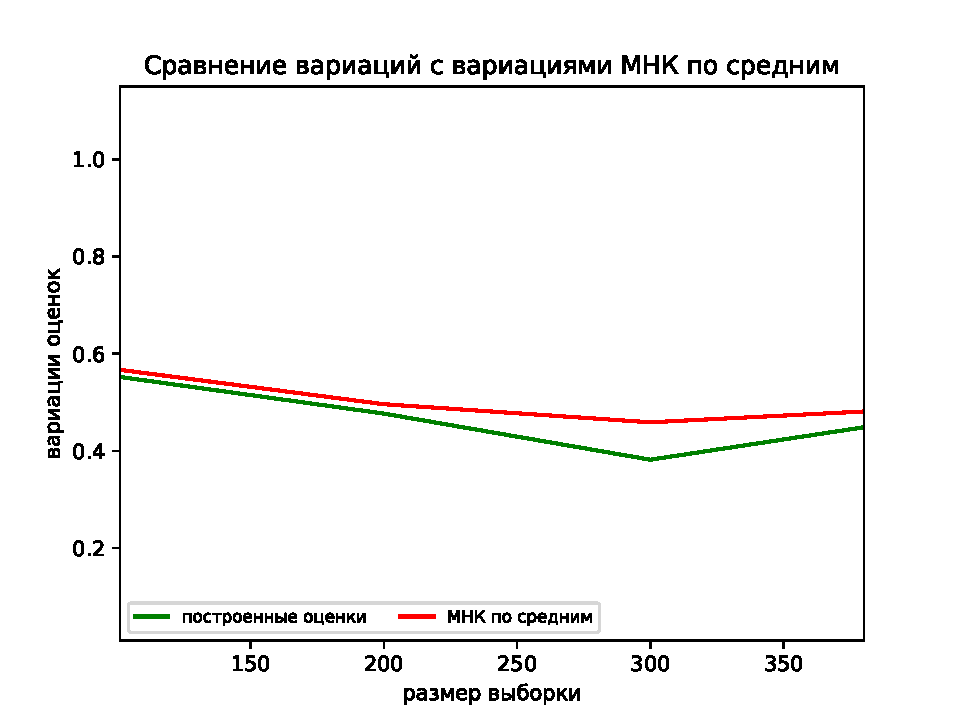
\includegraphics[width=100mm]{../images/OLS_GEM.pdf}
    \caption{Сравнение вариаций оценок\label{overflow}}
    \label{pic0}
\end{figure}
При сравнении графиков вариаций (рис.\ref{pic0}) можно сделать вывод, что ОМП дают лучший результат, 

\subsubsection{Эксперимент с полиномиальной регрессией}
Был проведен эксперимент с полиномиальной регрессией. Использовались те же параметры модели (таблица \ref{tab1}), объем выборки $N$ изменялся от 100 до 1000:
\begin{figure}[h!]
    \centering
    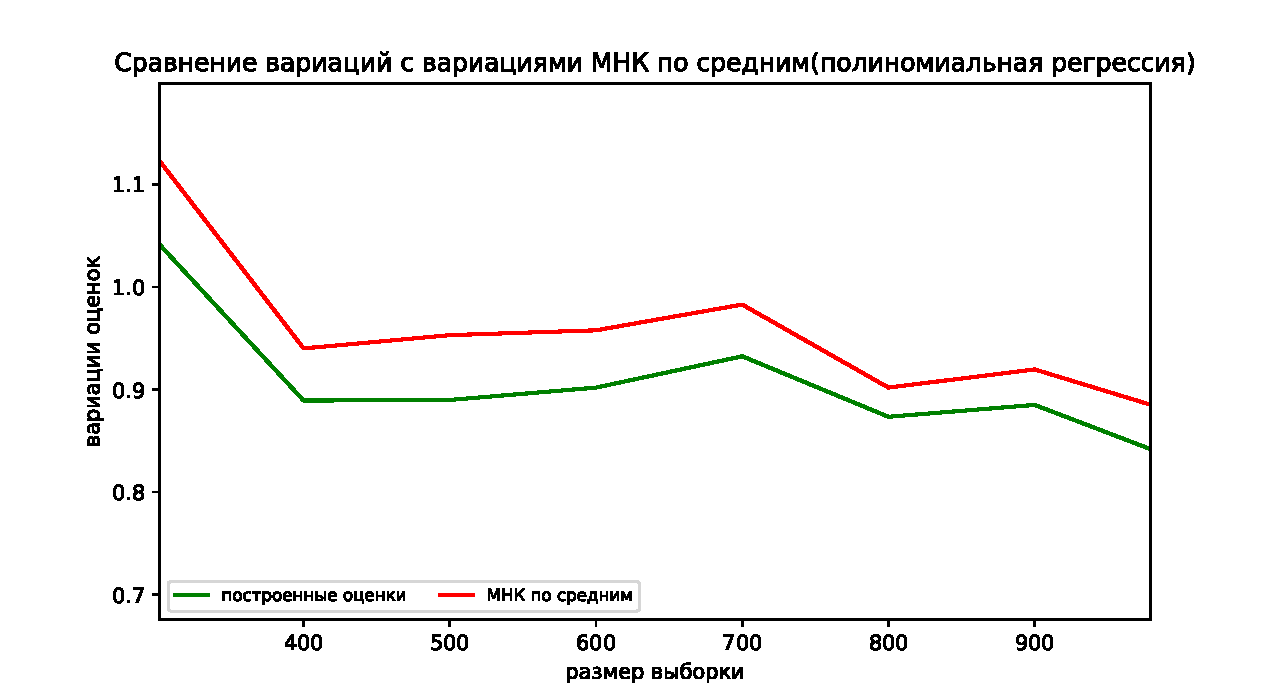
\includegraphics[width=150mm]{../images/polynomial.pdf}
    \caption{Вариации оценок в случае полиномиальной регрессии\label{overflow}}
    \label{pic3}
\end{figure}

Оба метода имели схожее поведение при изменении объема выборки, но построенные оценки максимального правдоподобия стабильно показывали лучший результат.

\newpage
\subsection{Эксперименты с изменением уровня переклассификации выборки для метода k-средних}\label{ss3_3_1}
В ходе преддипломной практики были построены эксперименты с изменением величины K для метода $K$-ближайших соседей, используемого в переклассификации.  

Объем выборки $N$ был постоянным: $N=500$. Использовалась модель линейной регрессии. Доля выбросов была постоянна и равнялась $\widetilde{\varepsilon}=0.08$. Параметры регрессии были постоянными и равнялись $\beta=(90,4)^T$. 
Регрессоры $x_i$ были из равномерного распределения $U(-5,5)$, ошибки эспериментов $\varepsilon_i\sim \mathcal{N}(0,16)$. Величина $K$ менялась от $10$ до $40$.
\begin{center}
    \captionof{table}{Параметры модели и оценок экспериментов с переклассификацией выборки}\label{tab1}
    \begin{tabular}{|p{5cm}|p{5cm}|}
        \hline
        \multicolumn{2}{|c|}{Параметры программы} \\
        \hline
        Переменная&значение\\
        \hline
        Размер выборки $N$& 500\\
        \hline
        Доля выбросов $\widetilde{\varepsilon}$& 0.08\\
        \hline
        Параметры регрессии $\beta$& $(90,4)$\\
        \hline
        Регрессоры $x_i$ & $\sim U(-5,5)$\\
        \hline
        $\varepsilon_i$&$\sim \mathcal{N}(0,16)$\\
        \hline
        $\eta_i$&$\sim \mathcal{N}(100,100)$\\
        \hline
        Величина $K$  &от $10$ до $40$\\
        \hline
    \end{tabular},
\end{center}

\begin{figure}[h!]
    \centering
    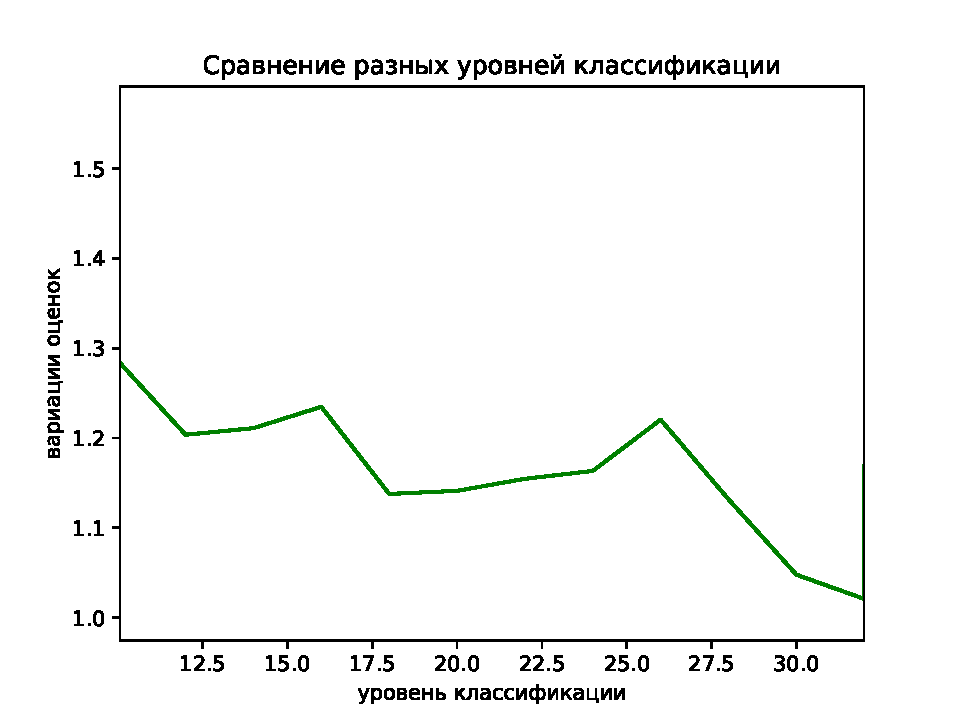
\includegraphics[width=100mm]{../images/different_recl_level.pdf}
    \caption{Зависимость вариаций от $K$ -- числа соседей, используемого в переклассификации выборки\label{overflow}}
    \label{pic1}
\end{figure}

В результате получилось, что при увеличении константы K точность оценки параметров растёт. 

\subsection{Эксперименты с изменением K для Least outlier factor, используемого в переклассификации}\label{ss3_3_2}
В ходе экспериментов была построена таблица, дающая хорошие значения K для выборки определенного объема с определенной длиной интервала, то есть такую величину $K$, при которой количество неверных классов после переклассификации не более чем такое количество до переклассификации (значения получены опытным путём).
 Доля выбросов была постоянна и равнялась $\widetilde{\varepsilon}=0.08$. Параметры регрессии были постоянными и равнялись $\beta=(90,4)^T$. 
Регрессоры $x_i$ были из равномерного распределения $U(-5,5)$, ошибки эспериментов $\varepsilon_i\sim \mathcal{N}(0,16)$.

\begin{center}
    \captionof{table}{Подходящие значения $K$ для выборки определенного объема с определенной длиной интервала}\label{tab2}
    \begin{tabular}{|p{5cm}|p{5cm}|p{5cm}|}
        \hline
        Объем выборки&длина интервала& величина $K$\\
        \hline
        1000 & 2.0 & 2\\
        1000 & 3.0 & 4\\
        1000 & 4.0 & 4\\

        3000 & 1.0 & 2\\
        3000 & 1.5 & 2\\
        3000 & 1.75 & 3\\
        3000 & 2.0 & 5\\
        3000 & 4.0 & 7\\

        10000 & 1.0 & 2\\
        10000 & 1.5 & 3\\
        10000 & 2.0 & 6\\
        10000 & 4.0 & 8\\
        \hline
    \end{tabular},
\end{center}
Пример получаемых в ходе экспериментов значений:
\begin{Verbatim}[fontsize=\scriptsize]
    modulated with outlier count: 189
    fit: classified
    wrong outliers: 181
    fit: reclassificator scored 0.928763 on learning set:
    fit: reclassified 10
    
    fit: classified
    
    Classes differ with/without outliers when without reclassification: 175
    Classes differ with/without outliers when with reclassification: 172
\end{Verbatim}

\newpage
\subsection{Сравнение вариаций с оценками без переклассификации}
Были проведены эксперименты для сравнения эмпирической вариации оценок максимального правдоподобия, когда использовалась вышеописанная переклассификация и когда не использовалась. При этом на каждой итерации выборка увеличивалась. 

Объем выборки $N$ изменялся от $N_1=100$ до $N_2=400$, при этом выборка дополнялась, а не генерировалась новая. Использовалась модель линейной регрессии. Доля выбросов была постоянна и равнялась $\widetilde{\varepsilon}=0.08$. Параметры регрессии были постоянными и равнялись $\beta=(90,4)^T$. 
Регрессоры $x_i$ были из равномерного распределения $U(-5,5)$, ошибки эспериментов $\varepsilon_i\sim \mathcal{N}(0,16)$. В методе, где использовалась переклассификация, величина $K$ выбиралась: $K=10$.
\vspace{3cm}
\begin{center}
    \captionof{table}{Параметры модели и оценок экспериментов}\label{tab1}
    \begin{tabular}{|p{5cm}|p{5cm}|}
        \hline
        \multicolumn{2}{|c|}{Параметры программы} \\
        \hline
        Переменная&значение\\
        \hline
        Размер выборки $N$& от 100 до 400\\
        \hline
        Доля выбросов $\widetilde{\varepsilon}$& 0.08\\
        \hline
        Параметры регрессии $\beta$& $(90,4)$\\
        \hline
        Регрессоры $x_i$ & $\sim U(-5,5)$\\
        \hline
        $\varepsilon_i$&$\sim \mathcal{N}(0,16)$\\
        \hline
        $\eta_i$&$\sim \mathcal{N}(100,100)$\\
        \hline
        В методе, с переклассификацией величина $K$& 10\\
        \hline
    \end{tabular},
\end{center}
\newpage
\begin{figure}[ht!]
    \centering
    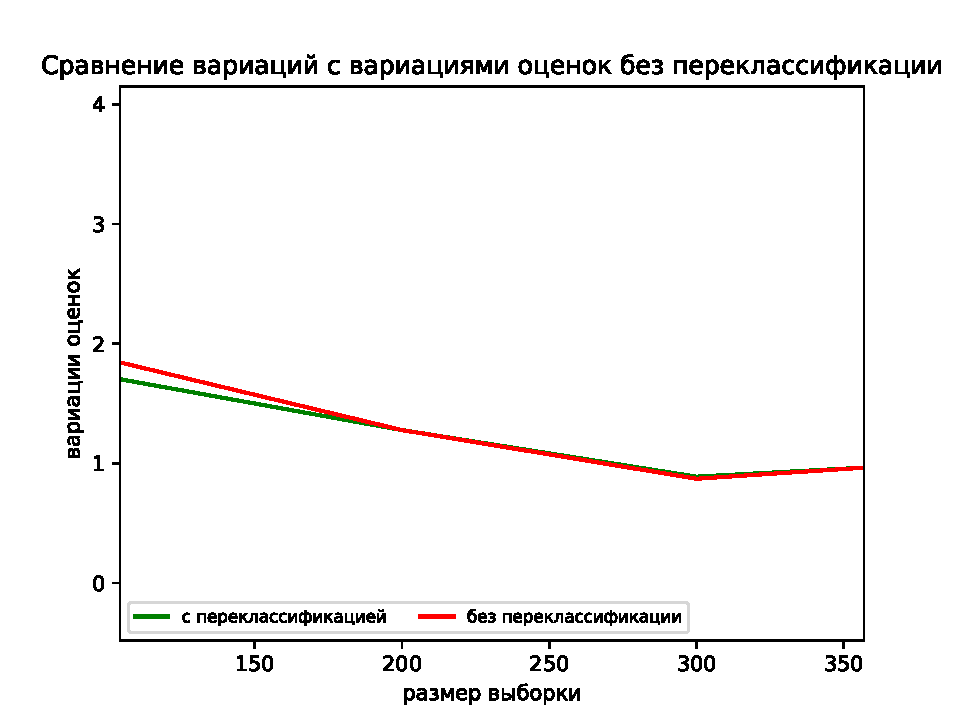
\includegraphics[width=100mm]{../images/on_off_recl.pdf}
    \caption{Сравнение вариаций оценок когда используется и не используется переклассификация\label{overflow}}
    \label{pic2}
\end{figure}

\newpage
